\section{Data}
The data used in this project is Dataset 2A: Climate and the Environment - General Measurements and Statistics. This dataset contains some general statistics and measurements of various aspects of the climate and the environment. It includes the following reports:
\begin{itemize}
    \item \textit{daily\_global\_weather}: Daily global weather from GHCN from January to October 2020
    \item \textit{greenhouse\_gas\_type} and \textit{greenhouse\_gas\_facility}: greenhouse gas emissions data reported by EPA, detailing the specific types of gas reported by facilities and general information about the facilities themselves. The dataset is made available through EPA’s GHGRP (Greenhouse Gas Reporting Program).
    \item \textit{us\_air\_quality}: air quality on a county level from approximately 4000 monitoring stations around the United States, reported from EPA’s Air Quality System (AQS)
\end{itemize}

Only the \textit{daily\_global\_weather}, \textit{greenhouse\_gas\_type}, and \textit{greenhouse\_gas\_facility} datasets were used in this analysis.

It should be noted that while the \textit{daily\_global\_weather} dataset collects weather from all over the world, the sampling in the data is heavily US-based. To prevent any bias in our analysis, we only focused on the US for our analysis. 


\begin{figure}
    \centering
    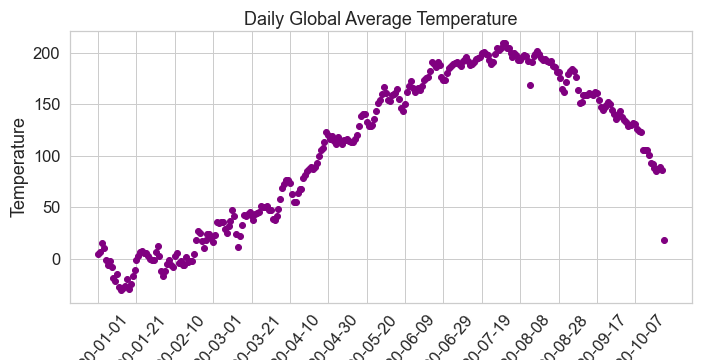
\includegraphics[width=\columnwidth]{figures/DailyAveTemp.png}
    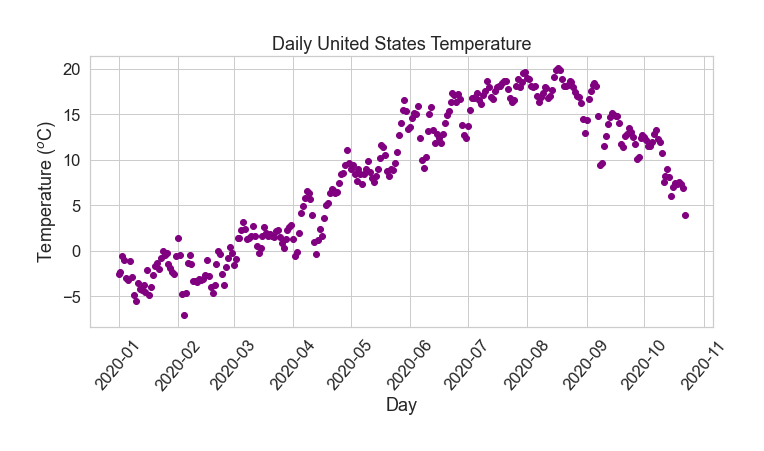
\includegraphics[width=\columnwidth]{figures/DailyAveUSTemp.png}
    \caption{Top: Daily Average Global Temperature generated by taking average temperature each day for all entries in \textit{daily\_global\_weather}\\Bottom:Daily Average US Temperature generated by taking average temperature each day for entries generated from the US in \textit{daily\_global\_weather}}
    \label{fig:US-bias}
\end{figure}
